\begin{figure}[htbp]
\centering
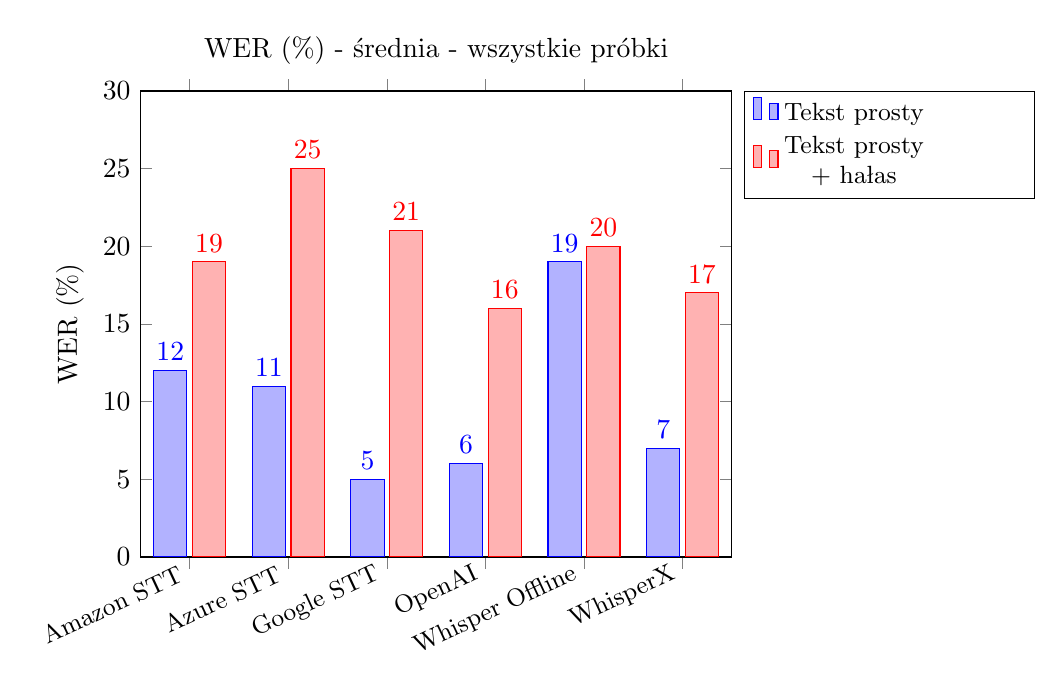
\begin{tikzpicture}
\begin{axis}[
    ybar=2pt,
    bar width=12pt,
    title={WER (\%) - średnia - wszystkie próbki},
    ylabel={WER (\%)},
    ymin=0, ymax=30,
    ytick={0,5,10,15,20,25,30},
    yticklabel={\pgfmathprintnumber[fixed,precision=0]{\tick}},
    symbolic x coords={
        Amazon STT,
        Azure STT,
        Google STT,
        OpenAI,
        Whisper Offline,
        WhisperX
    },
    xtick=data,
    enlarge x limits=0.10,
    x tick label style={
        rotate=25,
        anchor=east,
        font=\small
    },
    legend style={
        at={(1.02,1)},
        anchor=north west,
        font=\small,
        text width=3cm,
        align=left,
    },
    width=0.75\textwidth,
    height=7.5cm,
    nodes near coords,
    nodes near coords align={vertical},
    nodes near coords style={
        /pgf/number format/fixed,
        /pgf/number format/precision=0,
    }
]
\addplot coordinates {
    (Amazon STT,12)
    (Azure STT,11)
    (Google STT,5)
    (OpenAI,6)
    (Whisper Offline,19)
    (WhisperX,7)
};
\addplot coordinates {
    (Amazon STT,19)
    (Azure STT,25)
    (Google STT,21)
    (OpenAI,16)
    (Whisper Offline,20)
    (WhisperX,17)
};
\legend{Tekst prosty, {\shortstack{Tekst prosty\\+ hałas}}}
\end{axis}
\end{tikzpicture}
\caption{Porównanie przeskoków błędu WER pomiędzy tekstem prostym a tekstem z hałasem dla poszczególnych modeli ASR.}
\label{fig:wer_noise_jump_comparison}
\end{figure}
